\begingroup\hyphenpenalty=10000\relax
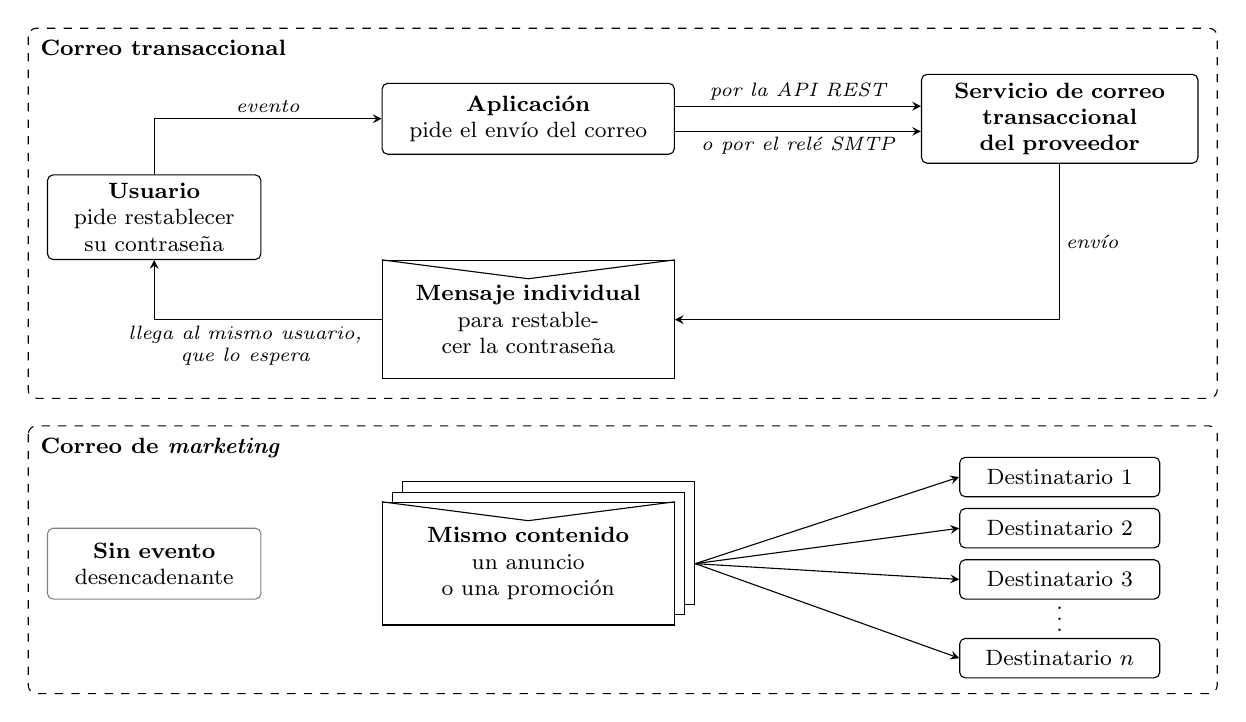
\begin{tikzpicture}[
  font=\footnotesize,
  actor/.style={draw, rounded corners=2pt, align=center, inner sep=3pt, minimum height=9mm},
  mensaje/.style={draw, fill=white, align=center, text width=35mm, inner xsep=3pt, inner ysep=3.2mm},
  cabecera/.style={font=\footnotesize\bfseries, anchor=north west, inner sep=0pt},
  rotulo/.style={font=\scriptsize\itshape, align=center, inner sep=2pt},
  ausente/.style={draw=gray, rounded corners=2pt, align=center, text width=25mm, minimum height=9mm, inner sep=3pt},
  destinatario/.style={draw, rounded corners=2pt, align=center, text width=24mm, minimum height=5mm, inner sep=2pt}
]
\node[cabecera] at (0,0) {Correo transaccional};
\draw[dashed, rounded corners=3pt] (-0.15,0.15) rectangle (14.95,-4.55);
\node[actor, text width=25mm] (usuario) at (1.45,-2.25) {\textbf{Usuario}\\ pide restablecer\\ su contraseña};
\node[actor, text width=35mm] (app) at (6.2,-1.0) {\textbf{Aplicación}\\ pide el envío del correo};
\node[actor, text width=33mm] (prov) at (12.95,-1.0) {\textbf{Servicio de correo transaccional del proveedor}};
\node[mensaje] (msj) at (6.2,-3.55) {\textbf{Mensaje individual}\\ para restablecer la contraseña};
\draw (msj.north west) -- ([yshift=-2.4mm]msj.north) -- (msj.north east);
\draw[-stealth] (usuario.north) |- node[rotulo, pos=0.75, above] {evento} (app.west);
\draw[-stealth] ([yshift=1.6mm]app.east) -- node[rotulo, above] {por la API REST} ([yshift=1.6mm]prov.west);
\draw[-stealth] ([yshift=-1.6mm]app.east) -- node[rotulo, below] {o por el relé SMTP} ([yshift=-1.6mm]prov.west);
\draw[-stealth] (prov.south) |- node[rotulo, pos=0.25, right] {envío} (msj.east);
\draw[-stealth] (msj.west) -| node[rotulo, pos=0.3, below] {llega al mismo usuario,\\ que lo espera} (usuario.south);
\draw[dashed, rounded corners=3pt] (-0.15,-4.9) rectangle (14.95,-8.3);
\node[cabecera] at (0,-5.05) {Correo de \textit{marketing}};
\node[ausente] (sinevento) at (1.45,-6.65) {\textbf{Sin evento}\\ desencadenante};
\foreach \c in {2,1} \node[mensaje] at ([xshift=\c*1.3mm, yshift=\c*1.3mm]6.2,-6.65) {\phantom{\textbf{Mismo contenido}}\\ \phantom{un anuncio}\\ \phantom{o una promoción}};
\node[mensaje] (masivo) at (6.2,-6.65) {\textbf{Mismo contenido}\\ un anuncio\\ o una promoción};
\draw (masivo.north west) -- ([yshift=-2.4mm]masivo.north) -- (masivo.north east);
\node[destinatario] (d1) at (12.95,-5.55) {Destinatario 1};
\node[destinatario] (d2) at (12.95,-6.2) {Destinatario 2};
\node[destinatario] (d3) at (12.95,-6.85) {Destinatario 3};
\node[anchor=base, inner sep=0pt] at (12.95,-7.51) {$\vdots$};
\node[destinatario] (dn) at (12.95,-7.85) {Destinatario $n$};
\foreach \d in {d1,d2,d3,dn} \draw[-stealth] ([xshift=2.6mm]masivo.east) -- (\d.west);
\end{tikzpicture}
\endgroup
